\documentclass[12pt,final]{article}
\usepackage[paperwidth=8.5in,left=0.5in,right=0.5in,top=1.0in,
            bottom=1.0in,paperheight=11.0in]{geometry}
\usepackage{enumitem}
\usepackage[breaklinks]{hyperref}
\hypersetup{pdfdisplaydoctitle=true,bookmarksnumbered=true,colorlinks=true,citecolor=black,linkcolor=blue,urlcolor=red,pdfstartview=FitH,pdfpagemode=UseNone}
\usepackage[sort&compress]{natbib}

\usepackage[nodisplayskipstretch]{setspace}
\doublespacing
\usepackage{times}
\usepackage{amssymb,amsmath,amsthm}
\usepackage{mathtools}
\usepackage{graphicx}
	\graphicspath{ {./graphics/} }
\usepackage{float}
\usepackage[labelsep=colon,small,singlelinecheck=off]{caption}
\usepackage[font+=small]{subcaption}
\usepackage{booktabs}
\usepackage{comment}

\makeatletter
\graphicspath{{figs/}}
\def\input@path{{tabs/}}
\def\bibfname{paper_bib.bib}
\makeatother

\title{The Pass-Through of Changes in Monetary Policy to Borrowing Costs}
\author{Daniel Posthumus}
\date{December 27, 2023}

\begin{document}
\vspace{-2in}
\maketitle
\vspace{-0.75in}
\section{Introduction}



The Federal Reserve conducts monetary policy in a variety of different ways, but the most common is by adjusting the Target Federal Funds Rate. By changing its policy rate, the Federal Reserve can change the costs of borrowing in the economy, although different interest rates respond to changes in the policy rate very differently. In order to test the pass-through of changes to the federal reserve policy rate (here we limit ourselves to conventional monetary policy making), we will engage in a three-pronged empirical approach: 1) a cross-sectional regression of changes in various borrowing costs in conjunction with the policy rate, 2) a vector auto-regressive (VAR) approach, and 3) a structural auto-regressive (SVAR) approach that borrows heavily from the work of Pétursson. \citep{Petursson2001}

\section{Literature Review}
\subsection{Pass-Through of Federal Funds Rate}
In 1995, Bernanke and Gertler looked inside the "Black Box"; in their seminal paper, they seek to understand in greater detail how monetary policy, specifically changes in the interest rate, affect the real economy \textit{through the credit channel}. \citep{Bernanke1995} In particular, we can conceive of two stages in the transmission channel capturing the pass-through of monetary policy shocks to borrowing costs. The first involves monetary policy's effects on the financial system, operating through the money markets to the bond market and the bank loan market. Then the second stage of this transmission is how shocks to the financial system affect the real economy, the effects that had been understood and thoroughly examined already prior to Bernanke and Gertler's work. Our paper is heavily inspired by Pétursson's work, and like him we focus on the first stage of the transmission mechanism, analyzing the pass-through effects of monetary policy shocks to the financial system. \citep{Petursson2001}


\section{Data}
Below is a table of the time-series data used in the regression analysis, with source, and available date ranges.\footnote{
\vspace{-0.1in}
\begin{itemize}
\itemsep-0.5em 
	\item The entries for "Dates Available" are in the following format: "MM/YYY". \\
"FRED" refers to the Federal Reserve Economic Data provided by the St. Louis Federal Reserve, located \href{https://fred.stlouisfed.org/}{here}.
	\item The term premium and expected short rate data are taken from Kim and Wright's three-factor DTSM yield decomposition. \citep{Kim2005} Data can be found \href{https://www.federalreserve.gov/data/three-factor-nominal-term-structure-model.htm}{here}.
	\item The effective federal funds rate and Wu-Xia Shadow Rate are taken from Wu and Xia's paper. \citep{Wu2016} Data can be found \href{https://www.atlantafed.org/cqer/research/wu-xia-shadow-federal-funds-rate}{here}.
	\item The four monetary policy shocks taken from a data replication file used in \citep{Acosta2022} are derived from two preceding papers. The news policy shock and expected federal funds shock are found in \citep{Nakamura2018}. Then the target and path shocks are found in \citep{Guerkaynak2005}. The replication data can be found \href{https://www.acostamiguel.com/research.html}{here}.
\end{itemize}}

\begin{table}[h!]
\caption{Time-Series Variables}
\noindent \begin{tabular}{|| l | l | l | l ||}
	\hline
	Series Name & Source & Dates Available \\
	\hline
	\textbf{General Economic Conditions} & & \\
	%GDP Implicit Price Deflator & FRED & 04/1947 - 04/2023 \\
	Core PCE Inflation & FRED & 01/1959 - 09/2023 \\ 
	%Homeownership Rate & FRED & 01/1965 - 07/2023 \\
	Real GDP & FRED & 01/1947 - 07/2023 \\
	CBOE VIX Index & FRED & 01/1990 - 12/2023 \\
	Unemployment Rate & FRED & 01/1948 - 10/2023 \\
	Labor Force Participation Rate & FRED & 01/1948 - 10/2023 \\
	\textbf{Measures of Borrowing Costs} & & \\ 
	30-year Mortgage Rate & FRED & 04/1971 - 10/2023 \\ 
	Moody's Seasoned AAA Corporate Bond Yield & FRED & 01/1983 - 11/2023 \\ 
	Treasury Debt Yields & US Dept. of Treasury & 01/1990 - 10/2023 \\
	Term Premium of Treasury Debt & \citep{Kim2005} & 01/1990 - 11/2023 \\ 
	Expect Short Rate & \citep{Kim2005} & 01/1990 - 11/2023 \\
	\textbf{Federal Reserve Data} & & \\
	%Upper Federal Funds Rate & FRED & Monthly & \\ 
	%Lower Federal Funds Rate & FRED & Monthly & \\ 
	Effective Federal Funds Rate & Atlanta Federal Reserve & 01/1960 - 02/2022 \\ 
	Wu-Xia Shadow Federal Funds Rate & Atlanta Federal Reserve & 01/1990 - 02/2022 \\ 
	FOMC Dummy Variable & \citep{Acosta2022} & 02/1995 - 09/2022 \\ 
	% FOMC and Federal Funds Rate Changes & Forbes & Monthly & \\
	\textbf{Monetary Policy Shock Data} & & \\
	News & \citep{Acosta2022} &  02/1995 - 09/2022 \\
	Expected Fed Funds & \citep{Acosta2022} & 02/1995 - 09/2022 \\ 
	Target & \citep{Acosta2022} & 02/1995 - 09/2022 \\
	Path & \citep{Acosta2022} & 02/1995 - 09/2022 \\ 
	\hline
\end{tabular}
\label{table:1}
\end{table}

Given the ranges of our data, we use a sample of the above time-series beginning in February 1995 and ending in September 2022.\footnote{Below are some notes about our data: 
\begin{itemize}
	\itemsep-0.5em 
	\item We use daily data wherever possible and collapse on the monthly averages to create monthly datasets. 
	\item In order to match quarterly-frequency data (i.e., Real GDP), we `fill in' the intervening empty months with the previous data. For example, if January 2019 (Q1 2019) registers a Real GDP growth of $g_1$\%, then February 2019 and March 2019 (until the Q2 observation in April 2019) will also have an observation for Real GDP growth of $g_1$\%.
	\item For each time-series we have crafted two types of change variables: change in levels and then percent change; this was calculated using the time-series operators of first lag and first-order difference in Stata. The exception is our quarterly variables, for which we calculated change by using their third-order lags and differences.
	\item We have constructed real measures of borrowing costs, by subtracting the monthly core PCE inflation from each month's observation of the borrowing cost.
	\item We have constructed the spreads of each borrowing costs against the 10-year Treasury Bond yield (which is often seen as the risk-free rate), simply by subtracting the 10-year yield from each borrowing cost. 
\end{itemize} } Now let's begin with a quick descriptive look at the data. From a cross-sectional perspective, clearly there is a strong positive correlation between the various measuring of borrowing costs, as the below matrix scatterplot graph shows us. However, the scatterplot shows that the strength of this correlation varies between relationships, although it does appear to be positive for all relationships. Next, we want to portray these relationships by drawing their time-series, as shown in the below graph. Clearly it appears that these rates move together. We can also observe that for these time-series are not stationary, or temporally homogenous. There is a clear downward trend of borrowing costs, independent of changes in the federal funds rate (represented by the shadow federal funds rate in the graph). \\
	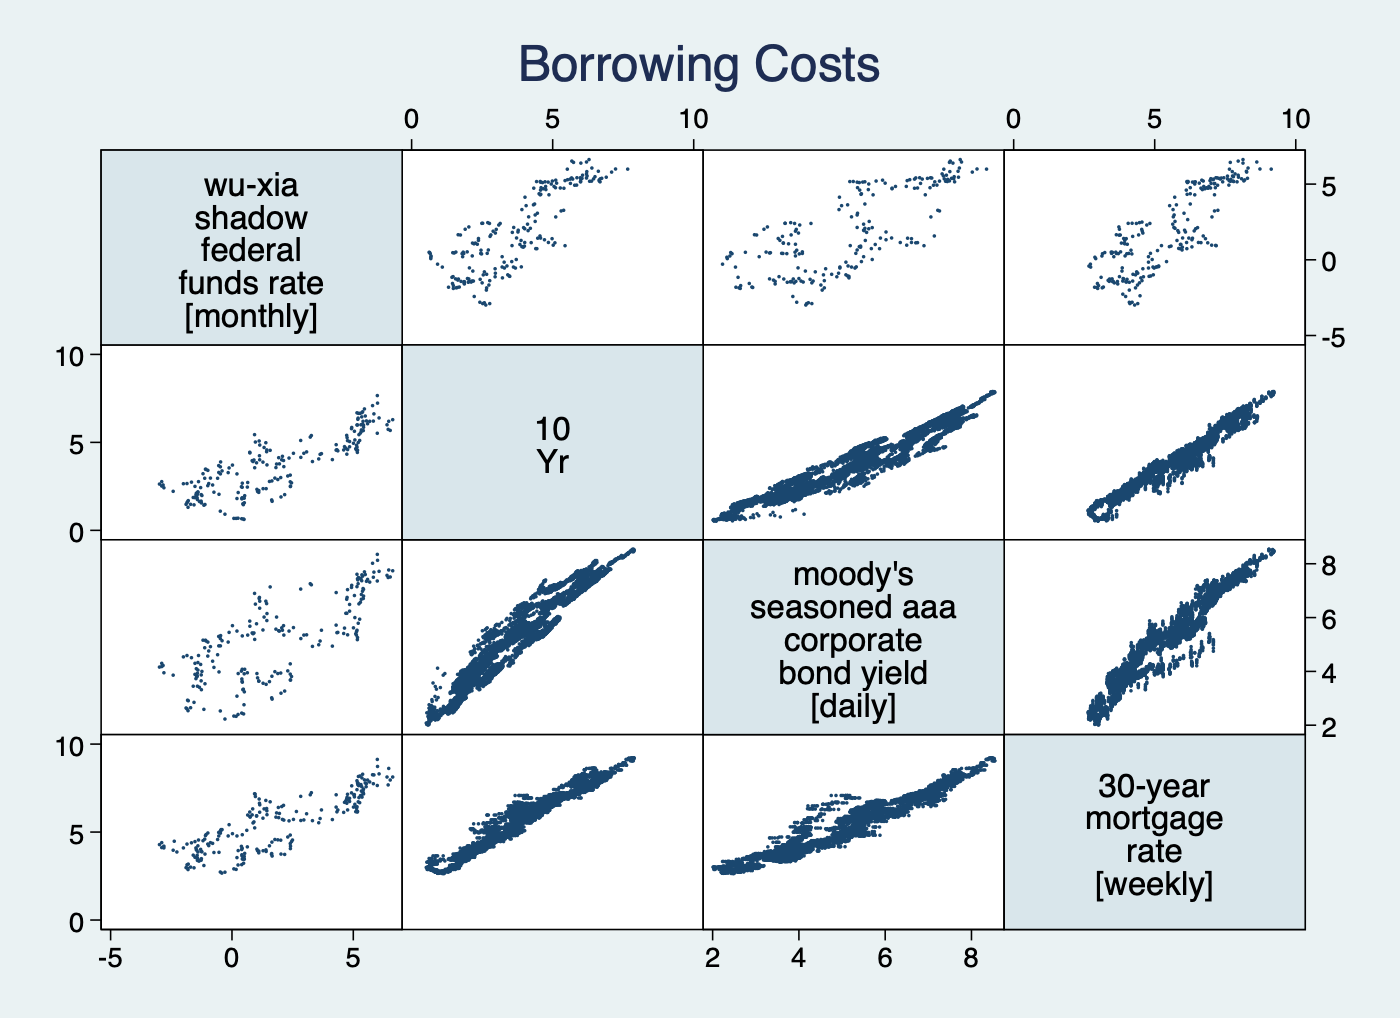
\includegraphics[width=3.75in]{matrix_graph.png} 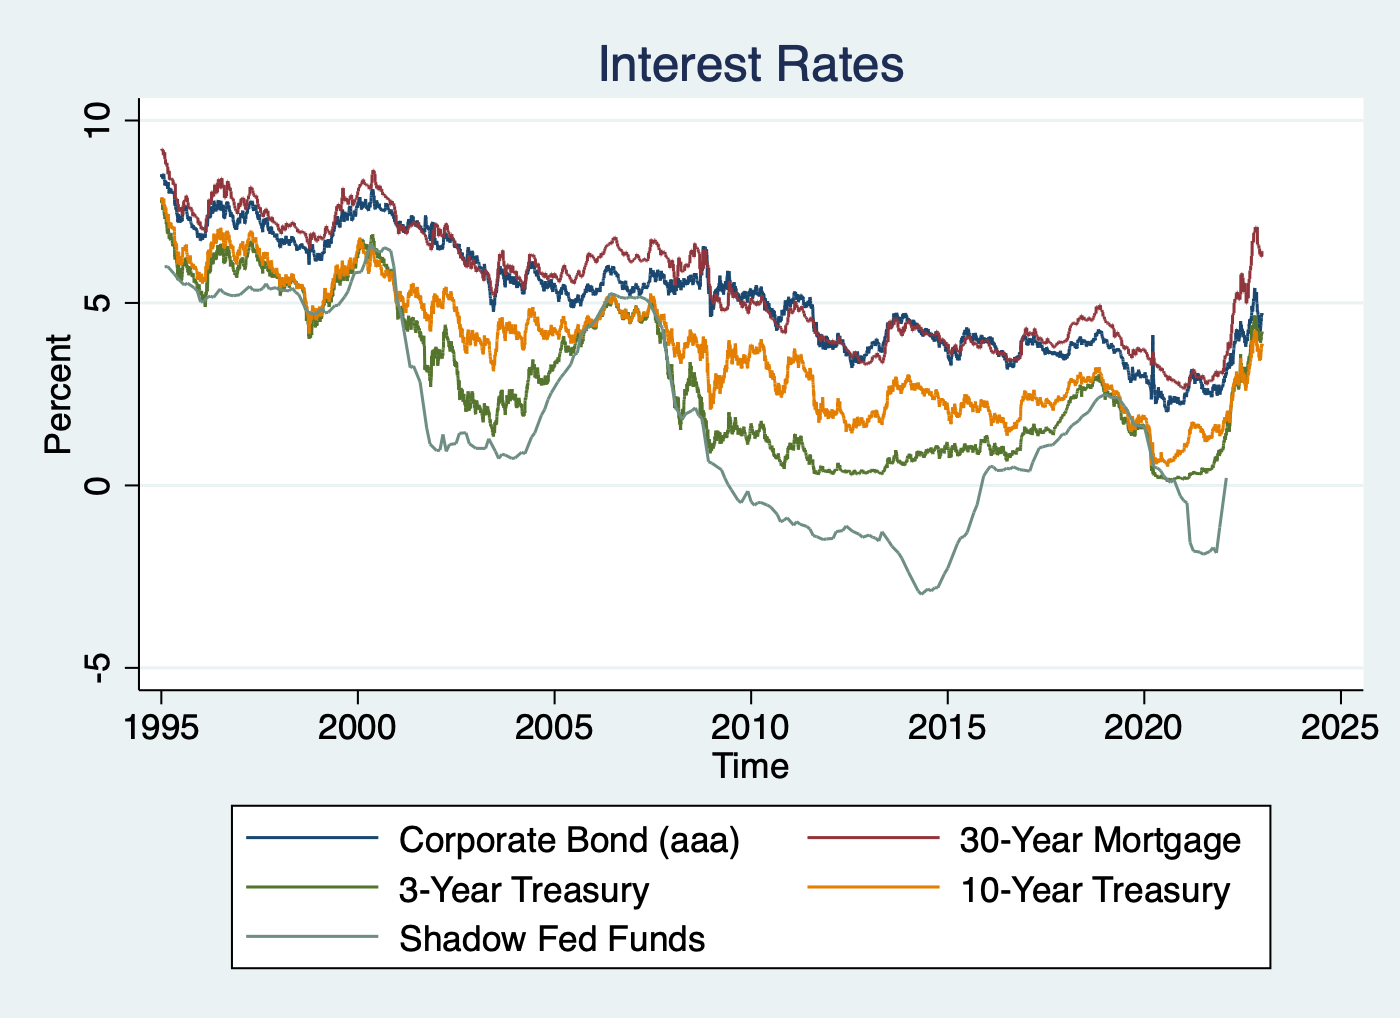
\includegraphics[width=3.75in]{all_rates.png}  \\
What if we de-trend the data from; specifically, creating a basic linear trend for each variable and then subtracting the value predicted by that linear trend from each observed value? Our data now appears nearly temporally homogenous, and we can see that the other borrowing costs follow more closely changes in the Shadow Federal Funds Rate. We have also plotted a graph showing the shocks from the Acosta paper, specifically the target rate shocks and the rate path shocks; we can see that not all changes in the shadow federal funds rate are accompanied by shocks, helping us to conceptualize the distinguish between surprise and non-surprise monetary policy changes. \\
	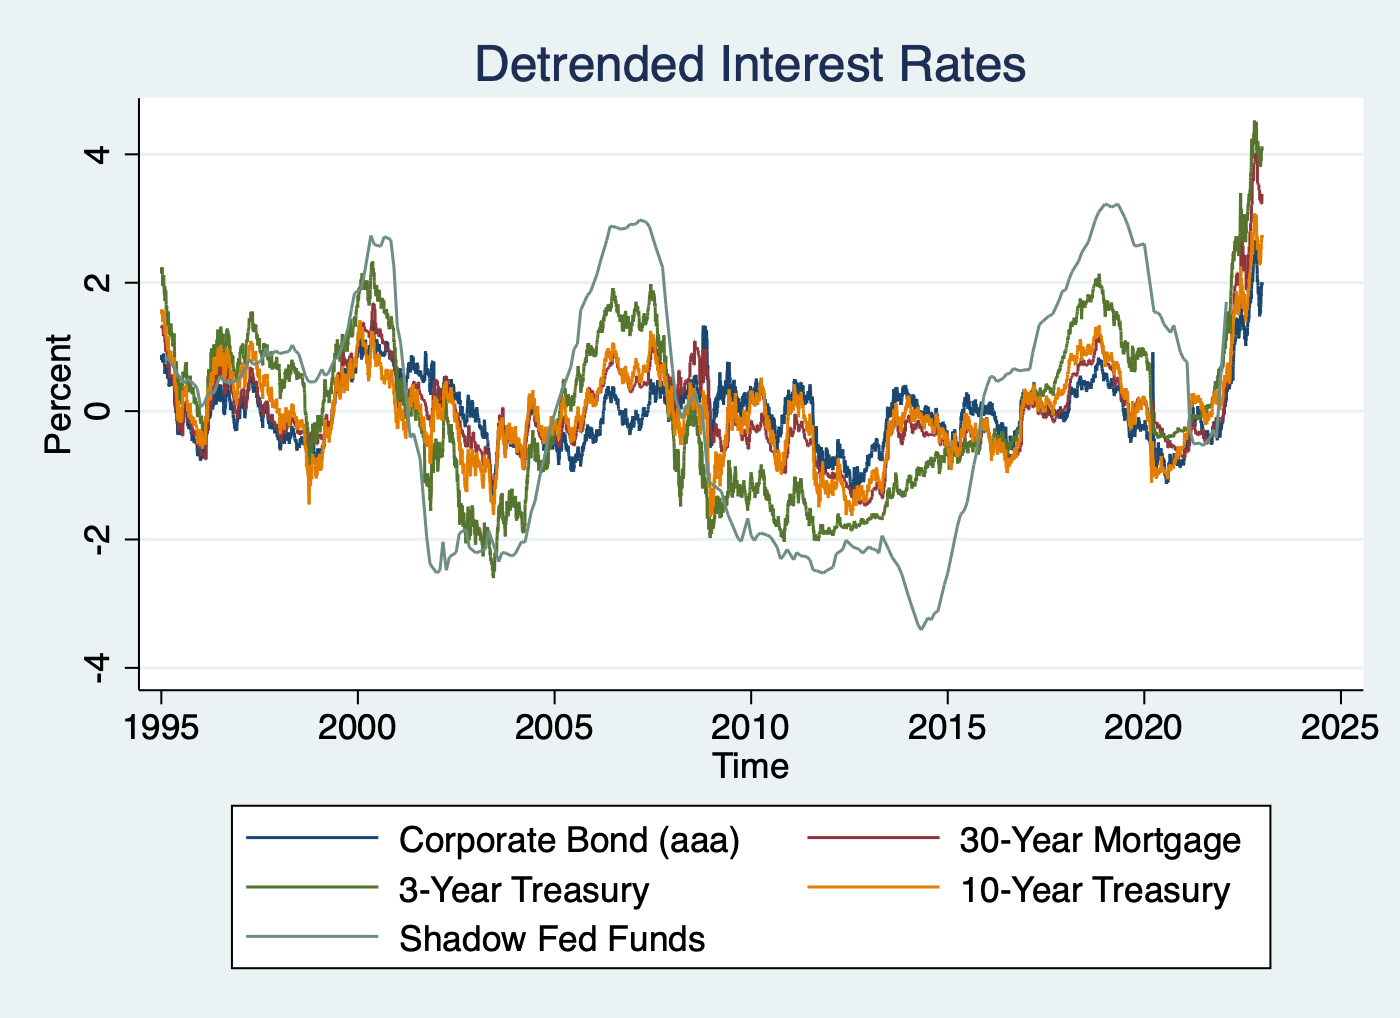
\includegraphics[width=3.75in]{detrend.png} 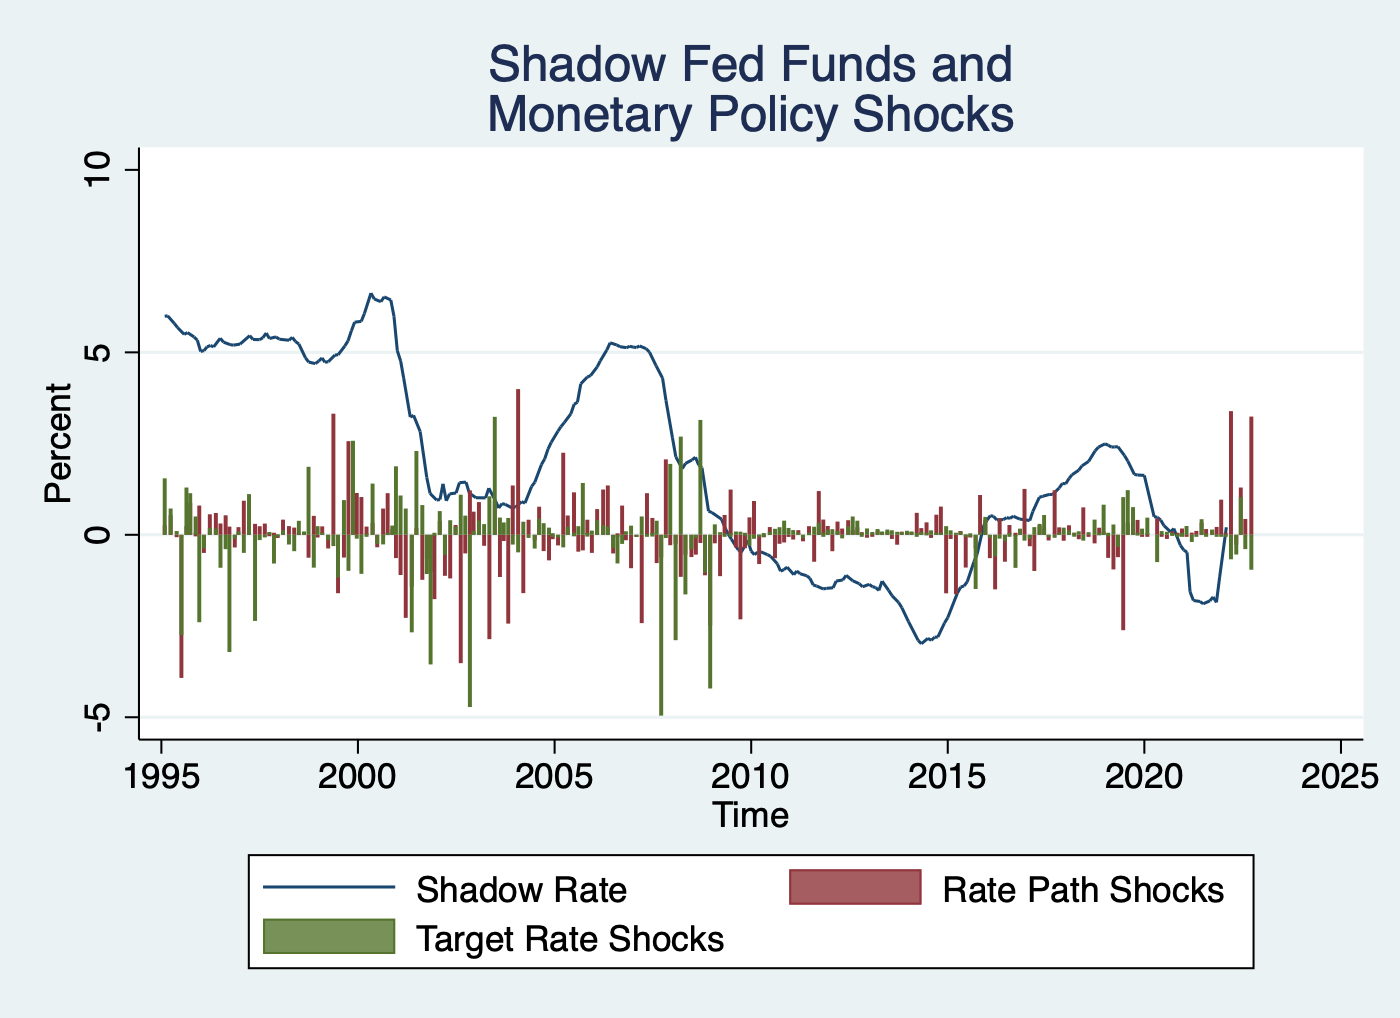
\includegraphics[width=3.75in]{shocks_time.png} \\

\section{Basic Regression Analysis}
Beginning with a cross-sectional approach, let's look at our basic regression results: \footnote{The macro conditions controlled for in the regressions denoted as such are core PCE inflation, the labor force participation rate, home ownership rate in the United States, real GDP growth, the unemployment rate, and the VIX index. \\ 
The de-trended data is merely the linear trend of each variable subtracted from the observed values. The regression estimates for the other two shocks in Acosta (2022), the news shocks and the shocks to the expected effective federal funds rate, are nearly identical to that of the target and path rate shocks.} \\
\begin{comment}
\begin{gather}
	y_t = \beta_{mp}MP + \beta_X\mathbf{X_t} + \epsilon_t \\
	(y_t - y_{t-1}) = \beta_{mp}MP + \beta_X(\mathbf{X_t} - \mathbf{X}_{t-1}) + \epsilon_t
\end{gather}
where $y_t$ is our borrowing cost of interest, $MP$ is the monetary policy dependent variable (which varies by specification).
\end{comment}
\begin{table}[!h]
\caption{Macroeconomic Factors' Relationship with Detrended Borrowing Costs}
\centering
\begin{tabular}{llllll}
\cline{1-6}
\multicolumn{1}{c}{} &
  \multicolumn{1}{|c}{3-Month} &
  \multicolumn{1}{c}{3-Year} &
  \multicolumn{1}{c}{10-Year} &
  \multicolumn{1}{c}{30-Year mortgage} &
  \multicolumn{1}{c}{Corporate bond} \\
\cline{1-6}
\multicolumn{1}{l}{Shadow rate} &
  \multicolumn{1}{|c}{0.648***} &
  \multicolumn{1}{c}{0.460***} &
  \multicolumn{1}{c}{0.147***} &
  \multicolumn{1}{c}{0.139***} &
  \multicolumn{1}{c}{0.005} \\
\multicolumn{1}{l}{} &
  \multicolumn{1}{|c}{(0.020)} &
  \multicolumn{1}{c}{(0.020)} &
  \multicolumn{1}{c}{(0.019)} &
  \multicolumn{1}{c}{(0.019)} &
  \multicolumn{1}{c}{(0.018)} \\
\multicolumn{1}{l}{Core PCE} &
  \multicolumn{1}{|c}{0.284***} &
  \multicolumn{1}{c}{0.403***} &
  \multicolumn{1}{c}{0.318***} &
  \multicolumn{1}{c}{0.298***} &
  \multicolumn{1}{c}{0.183***} \\
\multicolumn{1}{l}{} &
  \multicolumn{1}{|c}{(0.043)} &
  \multicolumn{1}{c}{(0.042)} &
  \multicolumn{1}{c}{(0.039)} &
  \multicolumn{1}{c}{(0.040)} &
  \multicolumn{1}{c}{(0.038)} \\
\multicolumn{1}{l}{Labor force participation} &
  \multicolumn{1}{|c}{-0.682***} &
  \multicolumn{1}{c}{-0.449***} &
  \multicolumn{1}{c}{-0.102***} &
  \multicolumn{1}{c}{-0.116***} &
  \multicolumn{1}{c}{0.055**} \\
\multicolumn{1}{l}{} &
  \multicolumn{1}{|c}{(0.031)} &
  \multicolumn{1}{c}{(0.030)} &
  \multicolumn{1}{c}{(0.029)} &
  \multicolumn{1}{c}{(0.029)} &
  \multicolumn{1}{c}{(0.027)} \\
\multicolumn{1}{l}{Home ownership rate} &
  \multicolumn{1}{|c}{0.064***} &
  \multicolumn{1}{c}{0.003} &
  \multicolumn{1}{c}{-0.027} &
  \multicolumn{1}{c}{0.044**} &
  \multicolumn{1}{c}{-0.050**} \\
\multicolumn{1}{l}{} &
  \multicolumn{1}{|c}{(0.023)} &
  \multicolumn{1}{c}{(0.023)} &
  \multicolumn{1}{c}{(0.022)} &
  \multicolumn{1}{c}{(0.022)} &
  \multicolumn{1}{c}{(0.021)} \\
\multicolumn{1}{l}{Real GDP growth} &
  \multicolumn{1}{|c}{1.315} &
  \multicolumn{1}{c}{-0.537} &
  \multicolumn{1}{c}{-0.375} &
  \multicolumn{1}{c}{-6.973***} &
  \multicolumn{1}{c}{-7.489***} \\
\multicolumn{1}{l}{} &
  \multicolumn{1}{|c}{(2.471)} &
  \multicolumn{1}{c}{(2.428)} &
  \multicolumn{1}{c}{(2.293)} &
  \multicolumn{1}{c}{(2.305)} &
  \multicolumn{1}{c}{(2.187)} \\
\multicolumn{1}{l}{Unemployment rate} &
  \multicolumn{1}{|c}{-0.131***} &
  \multicolumn{1}{c}{-0.144***} &
  \multicolumn{1}{c}{-0.050**} &
  \multicolumn{1}{c}{-0.085***} &
  \multicolumn{1}{c}{-0.046**} \\
\multicolumn{1}{l}{} &
  \multicolumn{1}{|c}{(0.023)} &
  \multicolumn{1}{c}{(0.023)} &
  \multicolumn{1}{c}{(0.021)} &
  \multicolumn{1}{c}{(0.022)} &
  \multicolumn{1}{c}{(0.020)} \\
\multicolumn{1}{l}{VIX Index (\% chg)} &
  \multicolumn{1}{|c}{0.011} &
  \multicolumn{1}{c}{-0.064} &
  \multicolumn{1}{c}{-0.002} &
  \multicolumn{1}{c}{0.074} &
  \multicolumn{1}{c}{0.099} \\
\multicolumn{1}{l}{} &
  \multicolumn{1}{|c}{(0.142)} &
  \multicolumn{1}{c}{(0.140)} &
  \multicolumn{1}{c}{(0.132)} &
  \multicolumn{1}{c}{(0.133)} &
  \multicolumn{1}{c}{(0.126)} \\
\multicolumn{1}{c}{Number of observations} &
  \multicolumn{1}{|c}{334} &
  \multicolumn{1}{c}{334} &
  \multicolumn{1}{c}{334} &
  \multicolumn{1}{c}{334} &
  \multicolumn{1}{c}{334} \\
\multicolumn{1}{c}{Adjusted R-squared} &
  \multicolumn{1}{|c}{0.868} &
  \multicolumn{1}{c}{0.823} &
  \multicolumn{1}{c}{0.473} &
  \multicolumn{1}{c}{0.491} &
  \multicolumn{1}{c}{0.175} \\
\cline{1-6}
\end{tabular}

\footnotesize{
*** p$<$.01, ** p$<$.05, * p$<$.1
}
\end{table}
 \\
Clearly, there is a strong positive correlation between the Shadow Rate and other borrowing costs, with or without macroeconomic controls (although the relationship does appear to become weaker when macroeconomic controls are included): all coefficients are positive and statistically significant except for the corporate bond detrended data with macro controls, unsurprising given that this rate appeared to be more independent of monetary policy in the above time-series graphs.

The regressions using first-differences of our outcome variables as the dependent variables and the monetary policy shock variables as the independent variables are more mixed; for news shocks and path shocks (which are highly correlated) we see similar, positive correlation, while the target and expected federal funds rates shocks show completely mixed results, with none statistically significant.

While interesting and important, these results are clearly limited in the conclusions we can draw. While the time-series are not purely Markovian (i.e., their current states entirely dependent on their past states), there is some auto-regressive properties, whether that's the lagged effects of monetary policy or through the signaling channel of updated economic news. We expect the state of borrowing costs and the economy yesterday to have some bearing on its state today. Inclusion of lagged variables becomes messy very quickly in cross-sectional approaches, as any semblance of collinearity goes out the window. Many articles in the literature seek to overcome this using structural approaches, such as the use of a Dynamic Term Structure Model (DTSM) in the work of Kim and Wright in decomposing changes in bond yields to isolate changes due to alterations to expected short rates and the term premia. \citep{Kim2005} We will use vector auto regression (VAR) techniques to try to overcome this empirical challenge.

\section{Structural Vector Auto Regression}
\subsection{Model Restrictions Identification}
In this paper, we will be using a Structural Vector Auto Regressive (SVAR) approach, as employed by Pétursson \citep{Petursson2001}. Following their lead, we divide the US financial system into four sub-markets, in order to create a set of variables representing our information set. Just as Pétursson does, we select the following time-series. First, for the policy rate set by the Fed, we will use the target federal funds rate, $r_t$, since this variable represents \textit{exactly} the policy rate of the Federal Reserve, unlike the effective federal funds rate and the shadow rate we used before. Second, there is the money market, for which we will also use the three month treasury bill rate, $m_t$. Third, to capture the bond market, we will use the market yield on a five-year US government bond, $g_t$.\footnote{Pétursson uses an indexed security; while he writes that in Iceland, his subject of study, 86\% of the total market value of government bonds were indexed, in the US inflation-indexed bonds make up only about 10\% of total marketable debt. \citep{Campbell2009}} Fourth and finally, to represent the sub-market of bank loans, we have selected the finance rate on personal loans at commercial banks for a 24-month loan, $b_t$. Below is a graph of all four of these time-series, as well as a graph of the de-trended (using the same linear de-trending process as above) series: \\
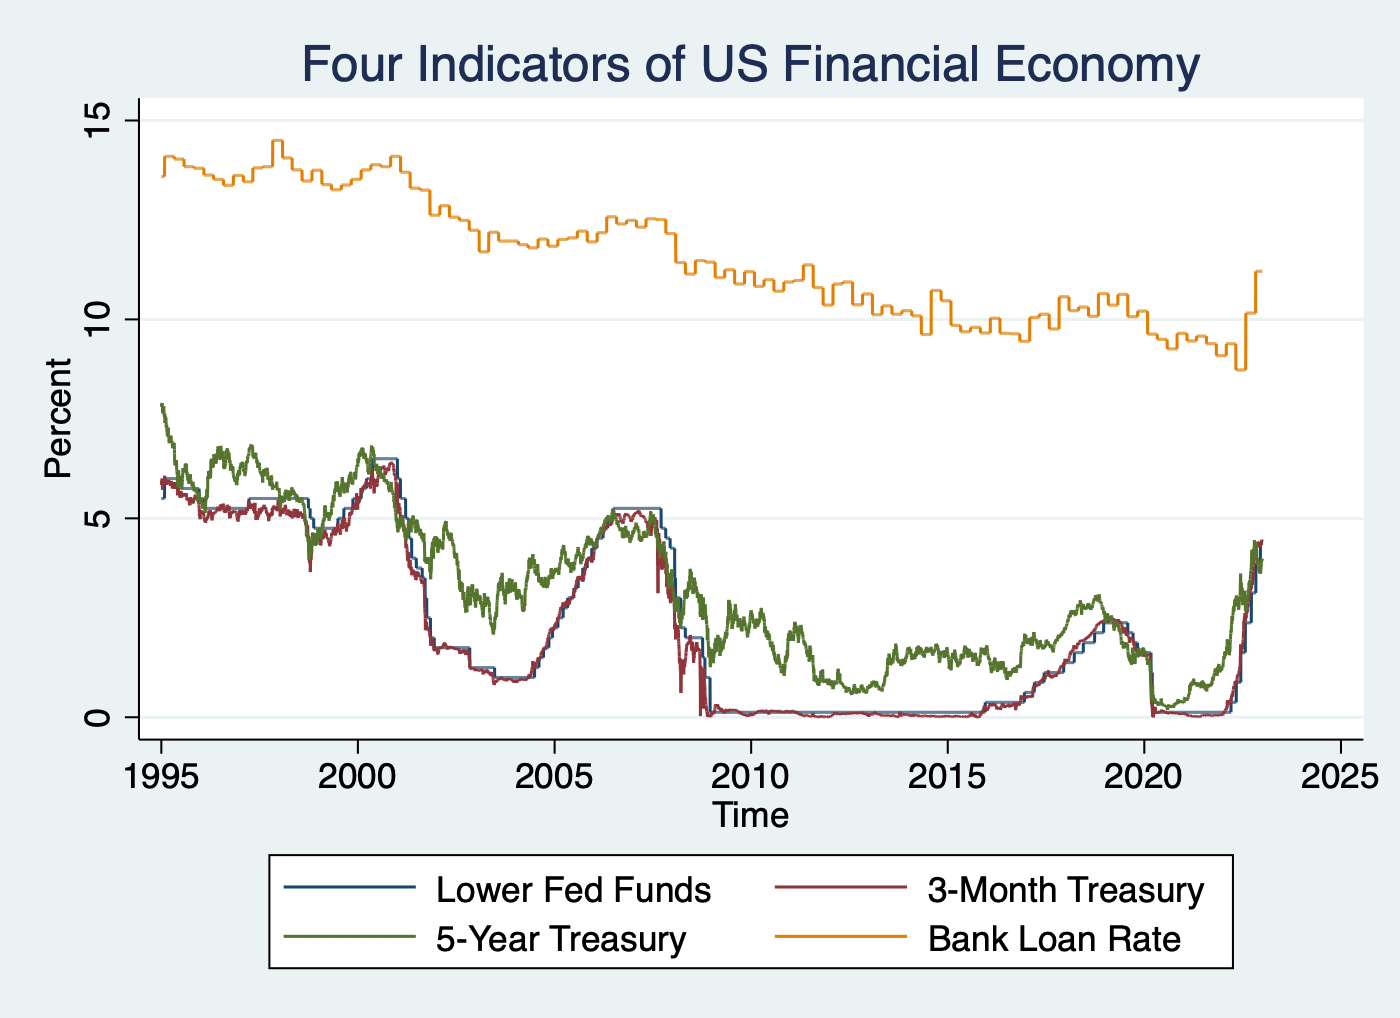
\includegraphics[width=3.75in]{svar_intro.png} 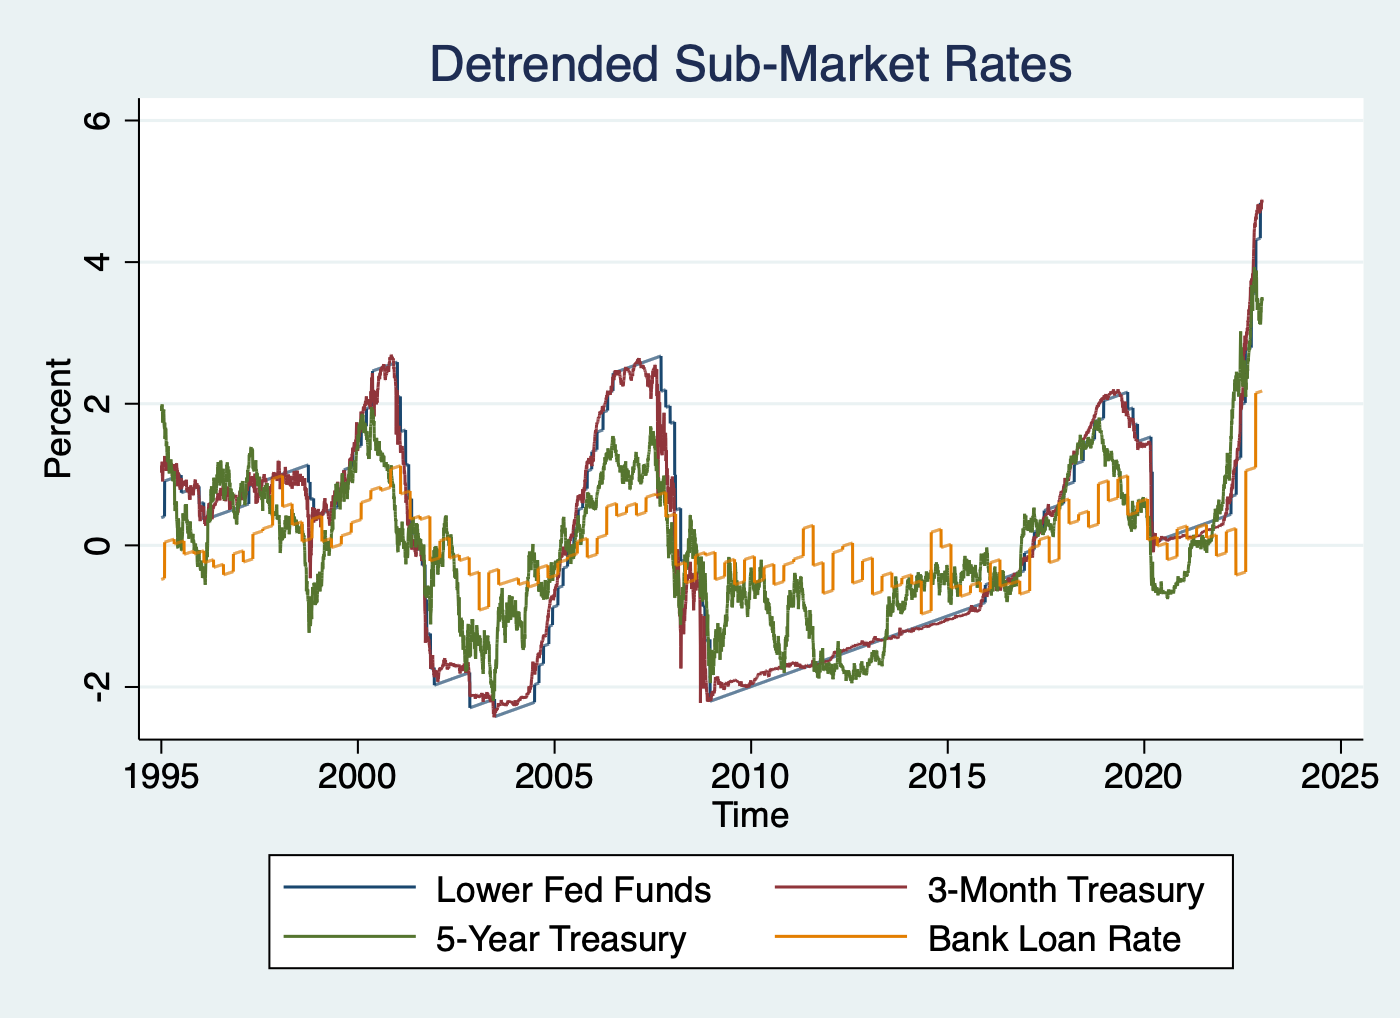
\includegraphics[width=3.75in]{svar_detrend.png} \\
We are using the same sample as our regression analysis, running from January, 1995 to September, 2022. We follow the work of Bernanke and Blinder (1992) in identifying monetary policy shocks, given by $\epsilon_{rt}$ as innovations to the target federal funds rate equation in the VAR model. \citep{Bernanke1990} Therefore to calculate innovations for each rate of interest, we merely construct a univariate auto-regressive model on their first-difference (to resolve the problem of stationarity), with lags determined by lag specification tests (whose results are reported in the Appendix). We then take the residual between the predicted value of the change in the rate for a given month and the observed one, resulting in the time-series seen below:  \\
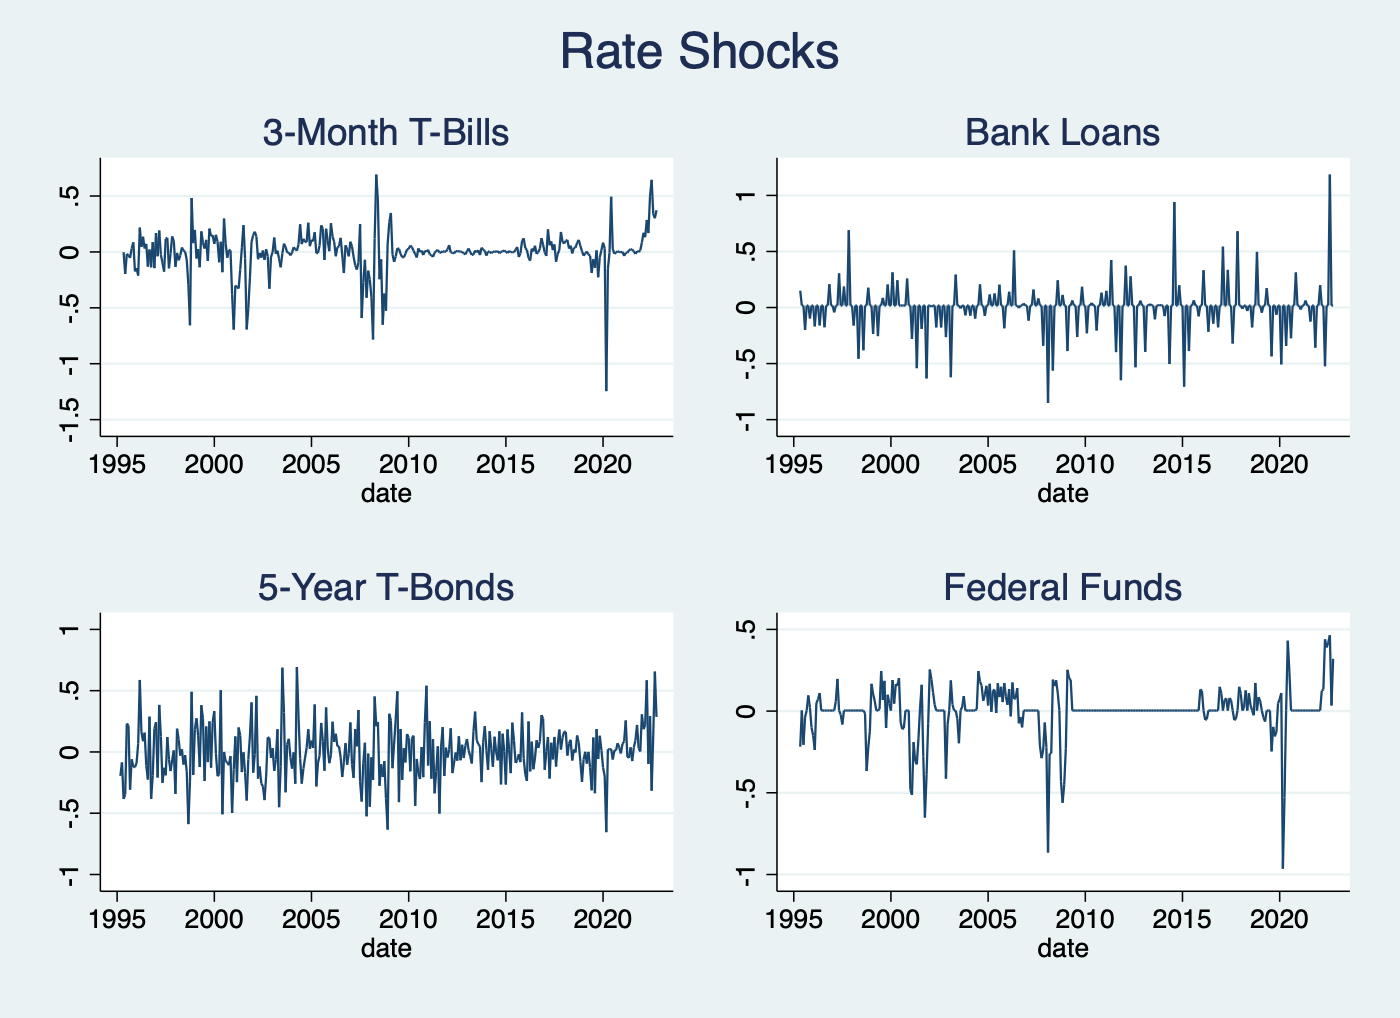
\includegraphics[width=3.75in]{shock_tsline.png} 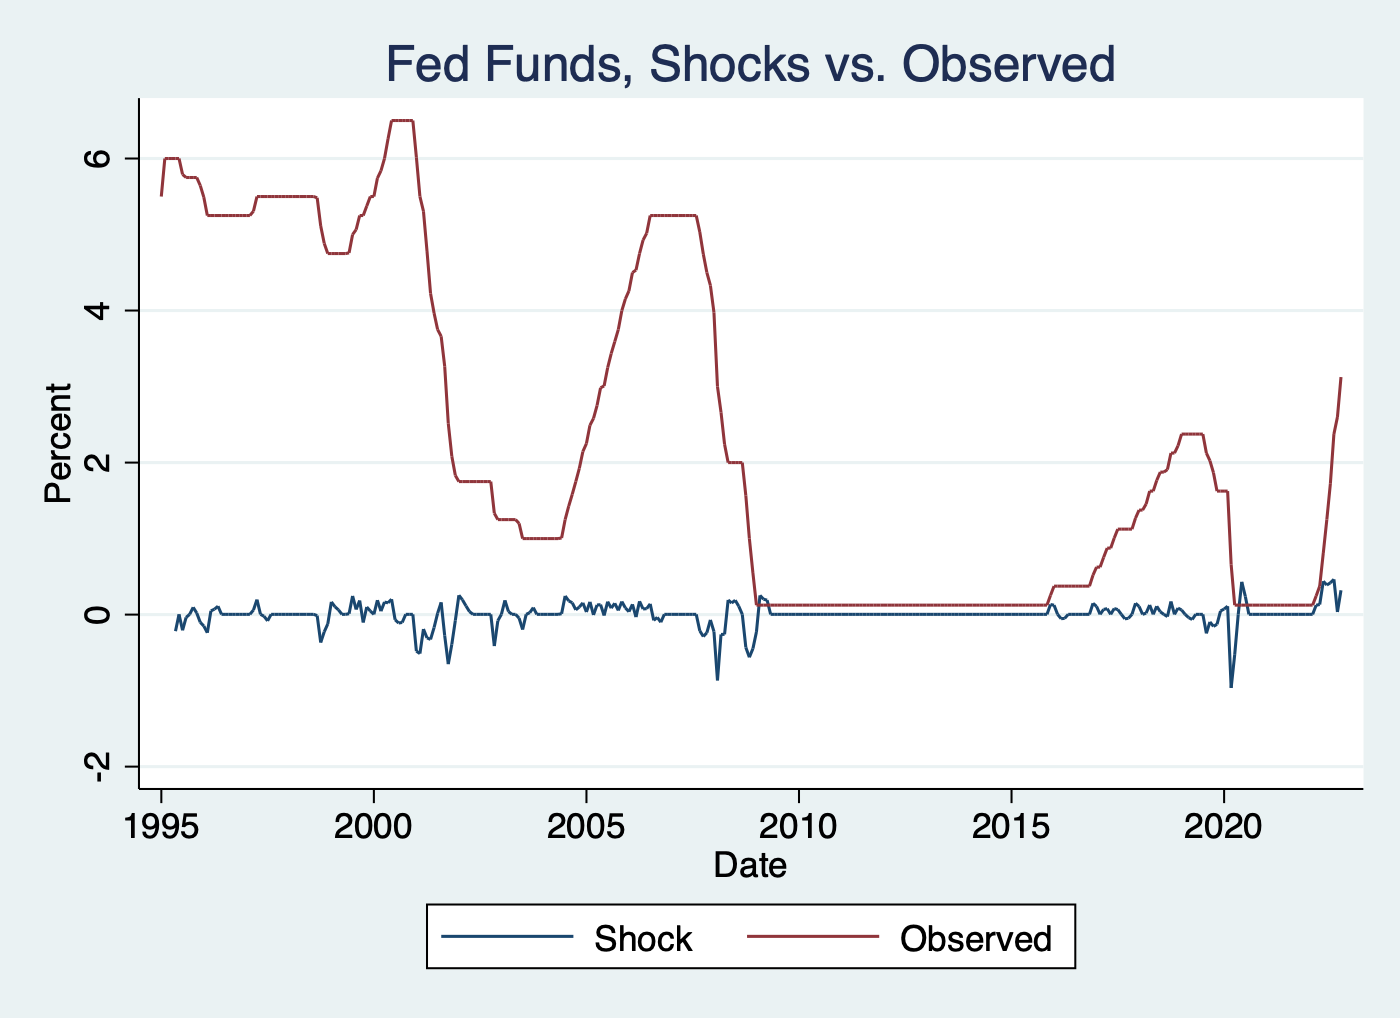
\includegraphics[width=3.75in]{shock_obs.png} \\
Although very noisy, we can see clear trends emerge. First, the bank loan data suffers the least variance of the four series, which confirms our intuition after seeing its de-trended time series plotted above. Next, looking at the scatter plot for the federal funds shock, we can clearly see the Zero Lower Bound, the drastic rate shocks immediately prior to the ZLB, post-COVID, and with the recent rate hikes--all differentiated from the more `routine' rate changes at other times (which may still be characterized by `shocks', but certainly at a lesser magnitude).

\subsection{Basic VAR Estimation}
Before proceeding to our structural VAR estimation, let's begin with a basic VAR of the first-difference in detrended rates. To estimate VAR, we must first find the most appropriate lag order for the VAR, which we will do using a sequence of likelihood ratio (LR) tests of the significance of each lag, shown here:
\begin{table}[!h]
\caption{Specification of the VAR}
\centering
\begin{tabular}{lllll}
\cline{1-5}
\multicolumn{1}{c}{} &
  \multicolumn{1}{|r}{AIC} &
  \multicolumn{1}{r}{SBIC} &
  \multicolumn{1}{r}{LL} &
  \multicolumn{1}{r}{LR} \\
\cline{1-5}
\multicolumn{1}{l}{k = 1} &
  \multicolumn{1}{|r}{-3.507} &
  \multicolumn{1}{r}{-3.276} &
  \multicolumn{1}{r}{596.943} &
  \multicolumn{1}{r}{343.100} \\
\multicolumn{1}{l}{k = 2} &
  \multicolumn{1}{|r}{-3.547} &
  \multicolumn{1}{r}{-3.132} &
  \multicolumn{1}{r}{619.559} &
  \multicolumn{1}{r}{45.233} \\
\multicolumn{1}{l}{k = 3} &
  \multicolumn{1}{|r}{-3.792} &
  \multicolumn{1}{r}{-3.192} &
  \multicolumn{1}{r}{675.743} &
  \multicolumn{1}{r}{112.367} \\
\multicolumn{1}{l}{k = 4} &
  \multicolumn{1}{|r}{-3.784} &
  \multicolumn{1}{r}{-2.999} &
  \multicolumn{1}{r}{690.395} &
  \multicolumn{1}{r}{29.306} \\
\cline{1-5}
\end{tabular}
\end{table}
 \\
Although the specification test results are mixed, the 3rd lag appears optimal. First, let's look at our auto-correlation plots: \\
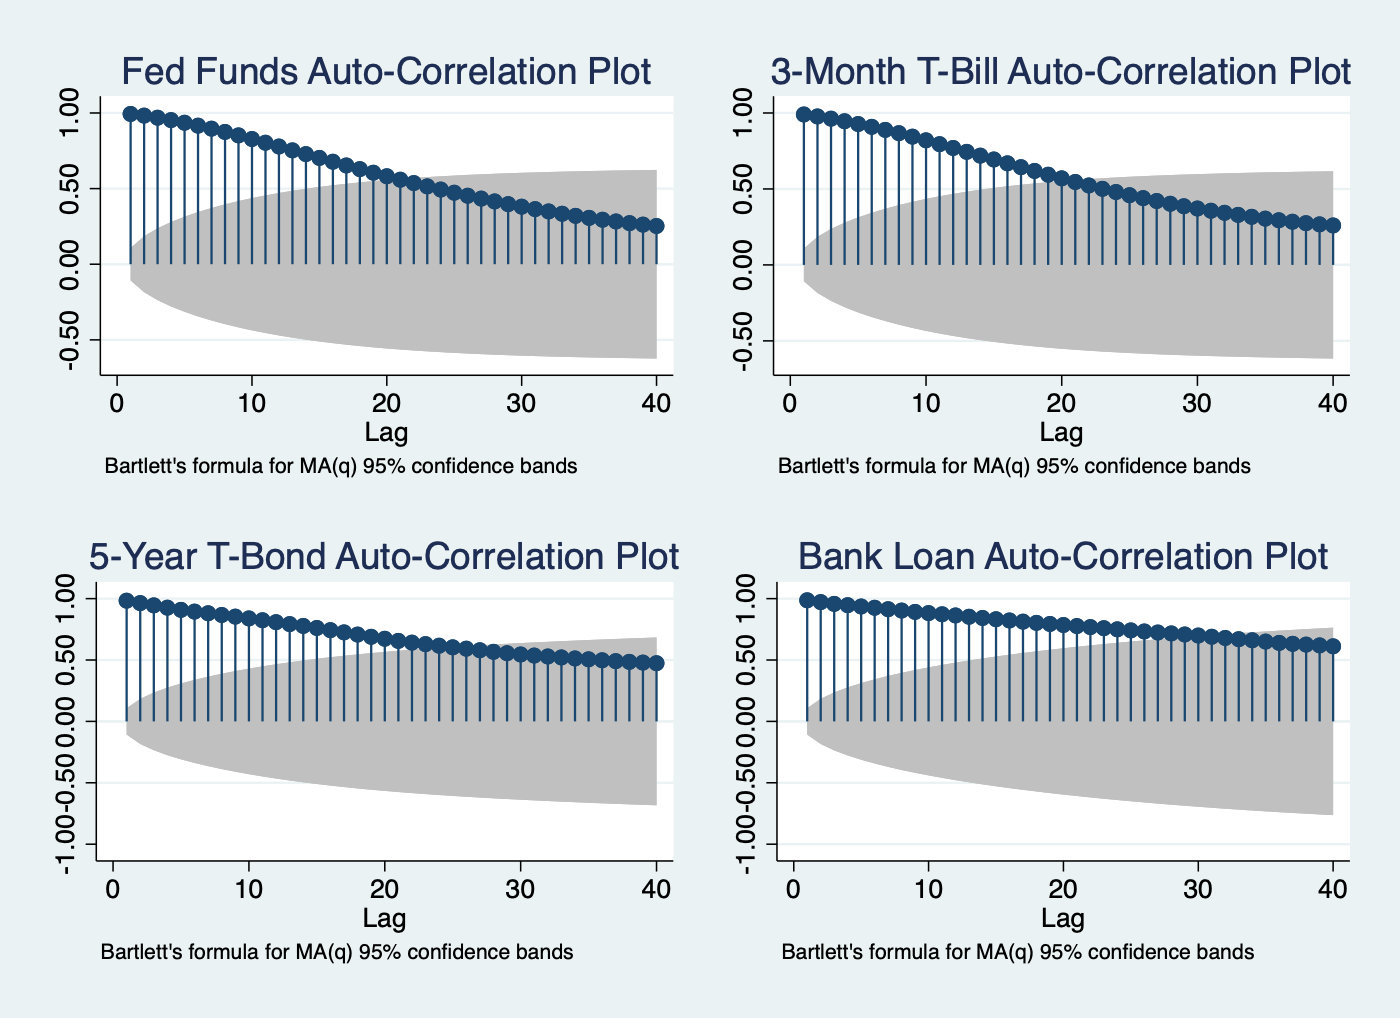
\includegraphics[width=3.75in]{var_ac.png} 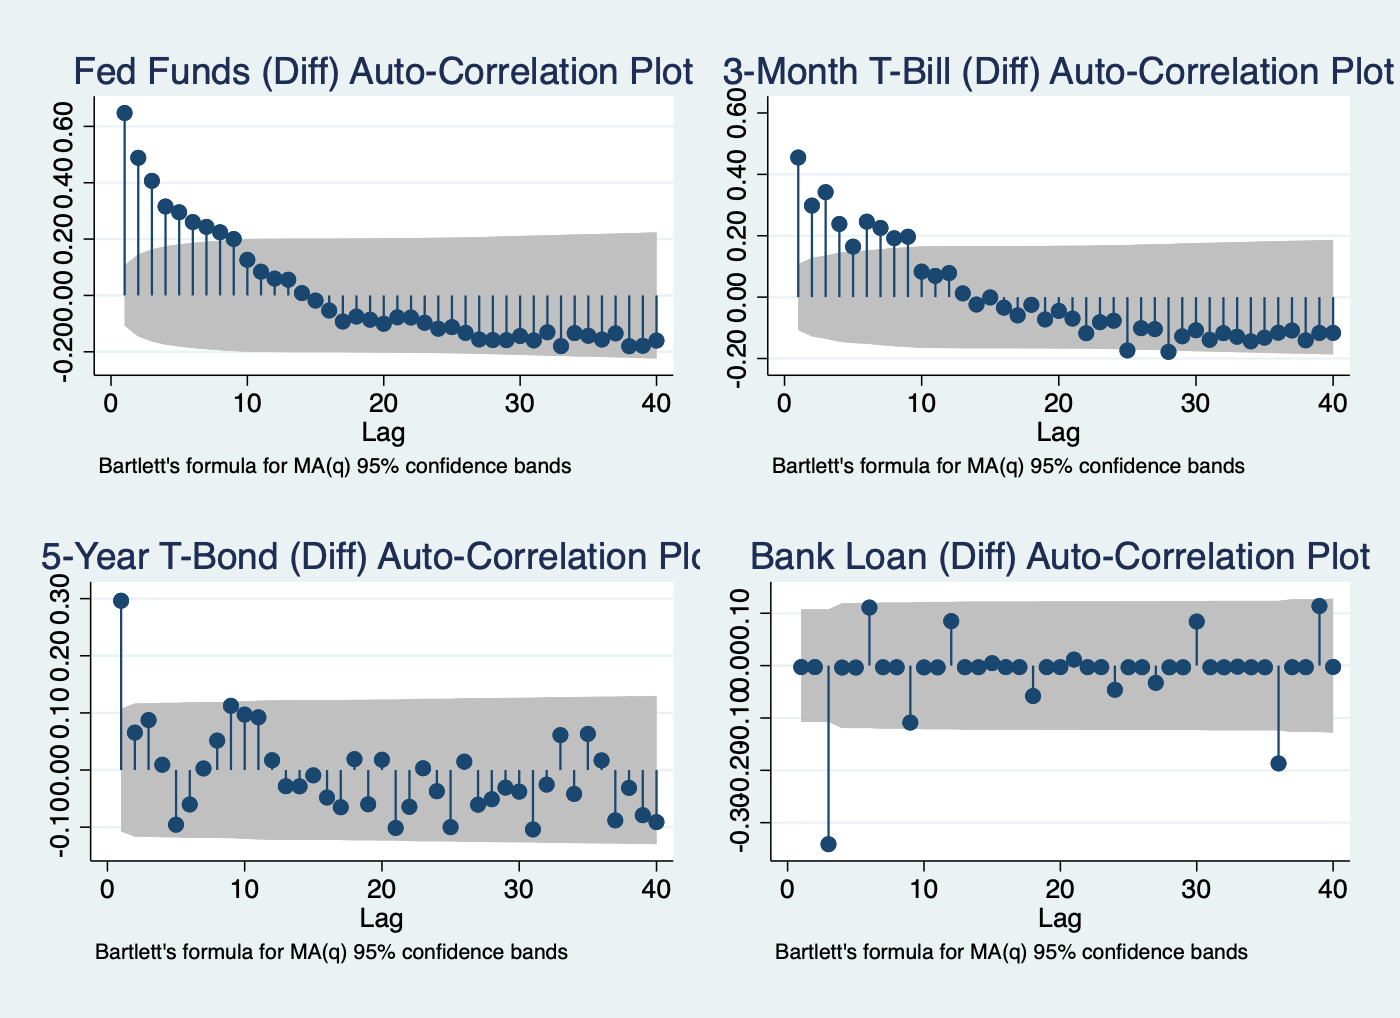
\includegraphics[width=3.75in]{var_ac_diff.png} \\
Clearly, there is too great of a deal of auto-correlation in the non-differenced data to effectively employ it in a VAR model, so we will proceed with the first-difference series, whose auto-correlations are plotted on the right and are much less serially correlated, if at all (certainly they don't seem so in the case of the 5-Year Bond and the Bank Loan series). Let's also check the results of a Dickey-Fuller Stationarity Test: \\
\begin{table}[!h]
\caption{Dickey-Fuller Stationarity Test Results}
\centering
\begin{tabular}{lll}
\cline{1-3}
\multicolumn{1}{c}{} &
  \multicolumn{1}{|r}{Test Statistic} &
  \multicolumn{1}{r}{P-Value} \\
\cline{1-3}
\multicolumn{1}{l}{Fed Funds} &
  \multicolumn{1}{|r}{-1.71} &
  \multicolumn{1}{r}{0.43} \\
\multicolumn{1}{l}{\quad Fed Funds (Diff)} &
  \multicolumn{1}{|r}{-4.99} &
  \multicolumn{1}{r}{0.00} \\
\multicolumn{1}{l}{\quad Fed Funds (Shock)} &
  \multicolumn{1}{|r}{-9.85} &
  \multicolumn{1}{r}{0.00} \\
\multicolumn{1}{l}{3-Month T-Bill} &
  \multicolumn{1}{|r}{-1.01} &
  \multicolumn{1}{r}{0.75} \\
\multicolumn{1}{l}{\quad 3-Month T-Bill (Diff)} &
  \multicolumn{1}{|r}{-5.36} &
  \multicolumn{1}{r}{0.00} \\
\multicolumn{1}{l}{\quad 3-Month T-Bill (Shock)} &
  \multicolumn{1}{|r}{-12.20} &
  \multicolumn{1}{r}{0.00} \\
\multicolumn{1}{l}{5-Year Bond} &
  \multicolumn{1}{|r}{-1.57} &
  \multicolumn{1}{r}{0.50} \\
\multicolumn{1}{l}{\quad 5-Year Bond (Diff)} &
  \multicolumn{1}{|r}{-8.46} &
  \multicolumn{1}{r}{0.00} \\
\multicolumn{1}{l}{\quad 5-Year Bond (Shock)} &
  \multicolumn{1}{|r}{-18.09} &
  \multicolumn{1}{r}{0.00} \\
\multicolumn{1}{l}{Bank Loan} &
  \multicolumn{1}{|r}{-4.12} &
  \multicolumn{1}{r}{0.00} \\
\multicolumn{1}{l}{\quad Bank Loan (Diff)} &
  \multicolumn{1}{|r}{-15.37} &
  \multicolumn{1}{r}{0.00} \\
\multicolumn{1}{l}{\quad Bank Loan (Shock)} &
  \multicolumn{1}{|r}{-18.25} &
  \multicolumn{1}{r}{0.00} \\
\cline{1-3}
\end{tabular}
\end{table}
 \\
We have achieved some measure of stationarity with the first-difference de-trended data as well as the shock data (we're able to reject the null hypothesis of the series having a `drift' for all 1st-difference and shock series, with p-values of 0.00); as stationarity is required, we're going to use the first-difference to run a basic VAR model that results in the following cumulative impulse response function graphs: \\
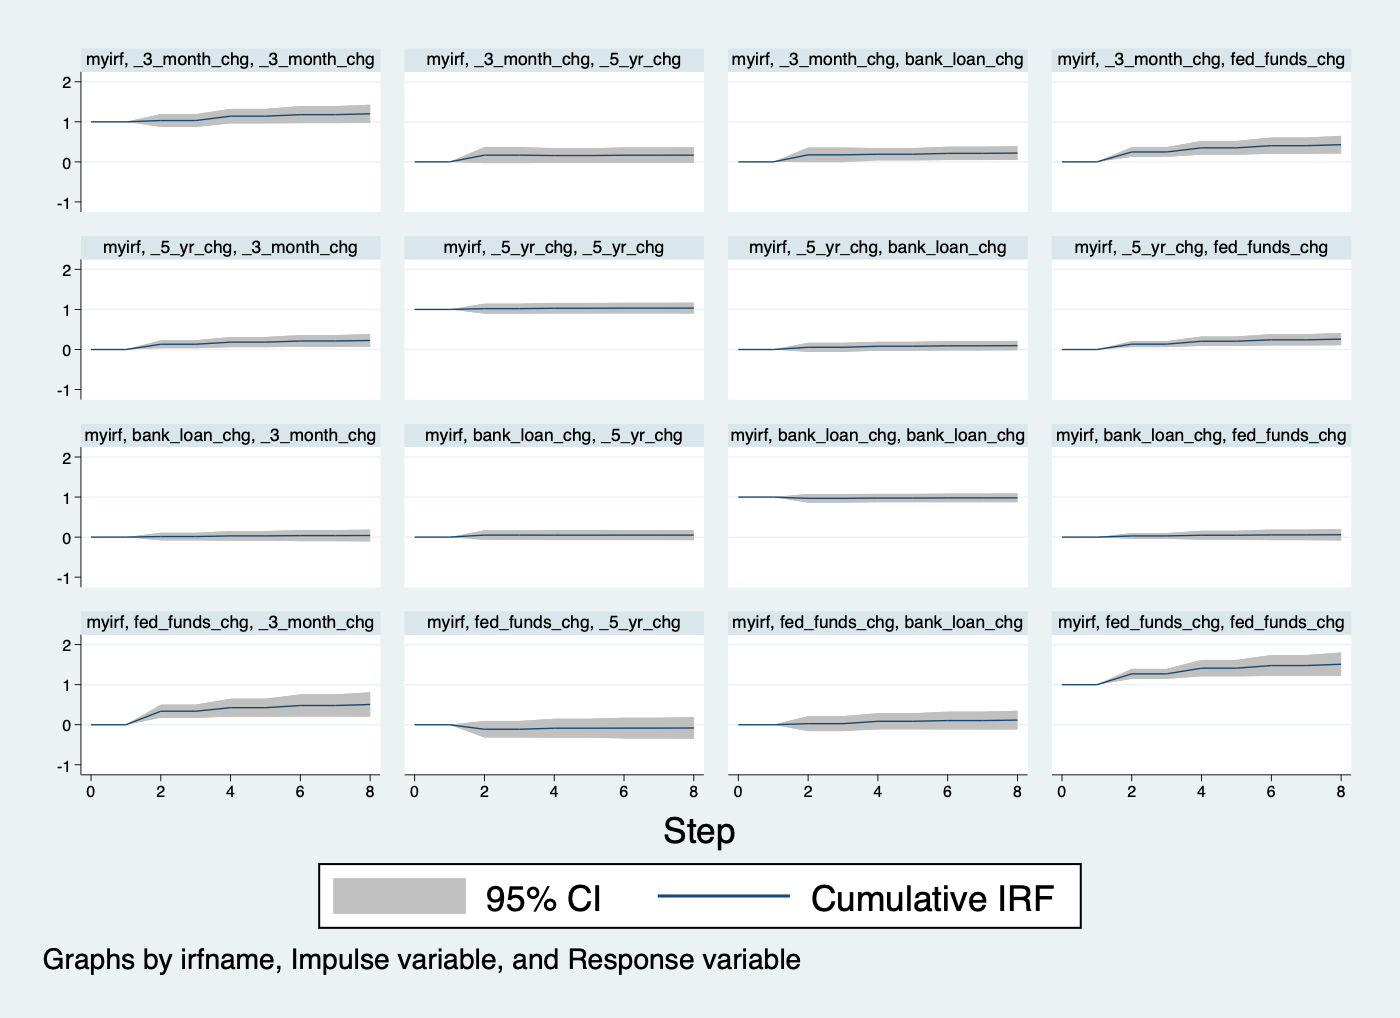
\includegraphics[width=5in]{var_basic.png} \\
As we would expect, there is a positive cumulative impulse response to changes across borrowing costs, with the sole exception of the 5-year Treasury Bond's response to the federal funds rate. We can also observe that the bank loan rate has by far the weakest response to shocks in other variables. In particular, as we would expect, the 3-month T-Bill is the most response to impulses from the federal funds rate, with the 5-year T-Bond being a little behind. This invites us to conduct a more rigorous analysis with a structural model.

\subsection{Structural Model Derivation}
Now let's derive the structural model. First, Pétursson models each of our three rates of interest, representing the three sub-markets of the financial system, as the dependent variable in a modeled relationship with the policy rate. \citep{Petursson2001} We begin with the money market rate, represented by the 3-month Treasury Bill Yield:
\begin{gather}
	e_{mt} = \alpha e_{rt} + \epsilon_{mt}
\end{gather}
where $\epsilon_{rt} = e_{rt}$ are monetary policy shocks, $\epsilon_{mt}$ is a shock to the very structure of the financial system (i.e., a change in how the financial system is operated in general), and finally $e_{mt}$ is the innovation to the money market rate resulting from the policy rate shock. We are not incorporating structural shocks into our analysis in this paper. Next, the relationship between the bond market rate (the 5-year Treasury Bond Yield) and the policy rate is given by:
\begin{gather}
	e_{gt} = \beta e_{rt} + \phi e_{mt} + \epsilon_{gt}
\end{gather}
where $e_{rt}$ and $e_{mt}$ is as defined above, $\epsilon_{gt}$ is a shock to the very structure of the bond system, and $e_{gt}$ is the innovation to the bond rate resulting from policy and money market shocks.\footnote{As Pétursson points out, the expectations hypothesis would suggest that the longer-term bond would be dependent entirely on the information communicated by the money market rate, i.e., that $\beta$ would be equal to 0; however, if $\beta \neq = 0$, then clearly there is some way that the policy rate shocks are affecting the bond market, \textit{other} than through affecting the money market.} Lastly, the bank loan rate (given by the commercial bank finance rate on personal loans) is assumed to follow from this equation:
\begin{gather}
	e_{bt} = f(e_{mct}) + \epsilon_{bt}, \quad \quad f' > 0, \quad \quad f = \rho e_{rt} + \mu e_{mt} + \gamma e_{gt} \\
	e_{bt} = \rho e_{rt} + \mu e_{mt} + \gamma e_{gt} + \epsilon e_{bt}
\end{gather}
where $f(e_{mct})$ is some always-increasing (hence the restriction that the first derivative always be greater than 0) function of $e_{mct}$, the innovations to the marginal cost of loan funding, $\epsilon_{bt}$ is a shock to the very structure of the bank loan marekt, and $e_{bt}$ is the innovation to the rate of bank loans resulting from these shocks. Equation (6) represents a direct relationship between the bank loan rate and shocks in the three preceding rates: the policy rate, the money market rate, and the bond rate, respectively. 

Resulting from assumptions about the nature of the basic model we outlined above, we can derive a matrix of correlations, $A_0$, that describes a Wold Causal Chain:\footnote{See Appendix for a more detailed description of the derivation of this Correlation matrix.}
\begin{gather}
	\begin{bmatrix}1&0&0&0\\-\alpha & 1 & 0 & 0 \\ -\beta & -\phi & 1 & 0 \\ -\rho & -\mu & -\gamma & 1 \end{bmatrix}
\end{gather}
where the coefficients in $A_0$ match those we defined in our linear model. The matrix $A_0$ thus is defined as a Wold causal chain structure between VAR innovations and \textit{structural} shocks.

\subsection{Reduced-Form Estimation}
To estimate our reduced-form model, which is as far as we will go in this paper, we estimate the coefficients in the matrix $A_0$ through the use of a dynamic factor model with the constraint of its coefficients following a Wold Causal Chain structure. This estimation leads us to the below estimated coefficients (in Table 5).
\begin{table}[!h]
\caption{Wold Causal Chain Estimation Results - Shocks}
\centering
\begin{tabular}{llll}
\cline{1-4}
\multicolumn{1}{c}{} &
  \multicolumn{1}{|r}{Coefficient} &
  \multicolumn{1}{r}{Std. error} &
  \multicolumn{1}{r}{p-value} \\
\cline{1-4}
\multicolumn{1}{l}{e.\_3\_month\_shock} &
  \multicolumn{1}{|r}{} &
  \multicolumn{1}{r}{} &
  \multicolumn{1}{r}{} \\
\multicolumn{1}{l}{\hspace{1em}L2e.\_3\_month\_shock} &
  \multicolumn{1}{|r}{-0.068} &
  \multicolumn{1}{r}{0.056} &
  \multicolumn{1}{r}{0.230} \\
\multicolumn{1}{l}{e.\_5\_yr\_shock} &
  \multicolumn{1}{|r}{} &
  \multicolumn{1}{r}{} &
  \multicolumn{1}{r}{} \\
\multicolumn{1}{l}{\hspace{1em}L2e.\_3\_month\_shock} &
  \multicolumn{1}{|r}{0.159} &
  \multicolumn{1}{r}{0.098} &
  \multicolumn{1}{r}{0.104} \\
\multicolumn{1}{l}{\hspace{1em}L2e.\_5\_yr\_shock} &
  \multicolumn{1}{|r}{-0.135} &
  \multicolumn{1}{r}{0.062} &
  \multicolumn{1}{r}{0.030} \\
\multicolumn{1}{l}{e.bank\_loan\_shock} &
  \multicolumn{1}{|r}{} &
  \multicolumn{1}{r}{} &
  \multicolumn{1}{r}{} \\
\multicolumn{1}{l}{\hspace{1em}L2e.\_3\_month\_shock} &
  \multicolumn{1}{|r}{0.130} &
  \multicolumn{1}{r}{0.087} &
  \multicolumn{1}{r}{0.135} \\
\multicolumn{1}{l}{\hspace{1em}L2e.\_5\_yr\_shock} &
  \multicolumn{1}{|r}{0.036} &
  \multicolumn{1}{r}{0.056} &
  \multicolumn{1}{r}{0.517} \\
\multicolumn{1}{l}{\hspace{1em}L2e.bank\_loan\_shock} &
  \multicolumn{1}{|r}{-0.029} &
  \multicolumn{1}{r}{0.056} &
  \multicolumn{1}{r}{0.600} \\
\multicolumn{1}{l}{\_3\_month\_shock} &
  \multicolumn{1}{|r}{} &
  \multicolumn{1}{r}{} &
  \multicolumn{1}{r}{} \\
\multicolumn{1}{l}{\hspace{1em}fed\_funds\_shock} &
  \multicolumn{1}{|r}{0.765} &
  \multicolumn{1}{r}{0.050} &
  \multicolumn{1}{r}{0.000} \\
\multicolumn{1}{l}{\hspace{1em}Intercept} &
  \multicolumn{1}{|r}{-0.000} &
  \multicolumn{1}{r}{0.007} &
  \multicolumn{1}{r}{0.984} \\
\multicolumn{1}{l}{\_5\_yr\_shock} &
  \multicolumn{1}{|r}{} &
  \multicolumn{1}{r}{} &
  \multicolumn{1}{r}{} \\
\multicolumn{1}{l}{\hspace{1em}fed\_funds\_shock} &
  \multicolumn{1}{|r}{0.180} &
  \multicolumn{1}{r}{0.080} &
  \multicolumn{1}{r}{0.024} \\
\multicolumn{1}{l}{\hspace{1em}Intercept} &
  \multicolumn{1}{|r}{0.001} &
  \multicolumn{1}{r}{0.010} &
  \multicolumn{1}{r}{0.926} \\
\multicolumn{1}{l}{bank\_loan\_shock} &
  \multicolumn{1}{|r}{} &
  \multicolumn{1}{r}{} &
  \multicolumn{1}{r}{} \\
\multicolumn{1}{l}{\hspace{1em}fed\_funds\_shock} &
  \multicolumn{1}{|r}{0.164} &
  \multicolumn{1}{r}{0.074} &
  \multicolumn{1}{r}{0.027} \\
\multicolumn{1}{l}{\hspace{1em}Intercept} &
  \multicolumn{1}{|r}{0.000} &
  \multicolumn{1}{r}{0.010} &
  \multicolumn{1}{r}{0.983} \\
\multicolumn{1}{l}{/observable} &
  \multicolumn{1}{|r}{} &
  \multicolumn{1}{r}{} &
  \multicolumn{1}{r}{} \\
\multicolumn{1}{l}{\hspace{1em}var(e.\_3\_month\_shock)} &
  \multicolumn{1}{|r}{0.020} &
  \multicolumn{1}{r}{0.002} &
  \multicolumn{1}{r}{0.000} \\
\multicolumn{1}{l}{\hspace{1em}var(e.\_5\_yr\_shock)} &
  \multicolumn{1}{|r}{0.046} &
  \multicolumn{1}{r}{0.004} &
  \multicolumn{1}{r}{0.000} \\
\multicolumn{1}{l}{\hspace{1em}var(e.bank\_loan\_shock)} &
  \multicolumn{1}{|r}{0.037} &
  \multicolumn{1}{r}{0.003} &
  \multicolumn{1}{r}{0.000} \\
\cline{1-4}
\end{tabular}
\end{table}
 \\
We see very strong statistically significant coefficients, largely with positive signs (which we would expect). We do want to note, however, that while all variables of interest appear to have significant positive relationships with shocks to the federal funds rate, there is no such consistency in the estimation of the relationships \textit{between} borrowing costs and interest rates, which exhibit much more muddled significance. Of particular note is the weak relationship between the bank loans and 5-year bond; instead, our results suggest, the bank loan market appears most reactive to the money market (represented by the 3-month bond) and the Federal Reserve's policy rate.

The estimation of the structural VAR with such restriction yields the following cumulative impulse response function graph: \\
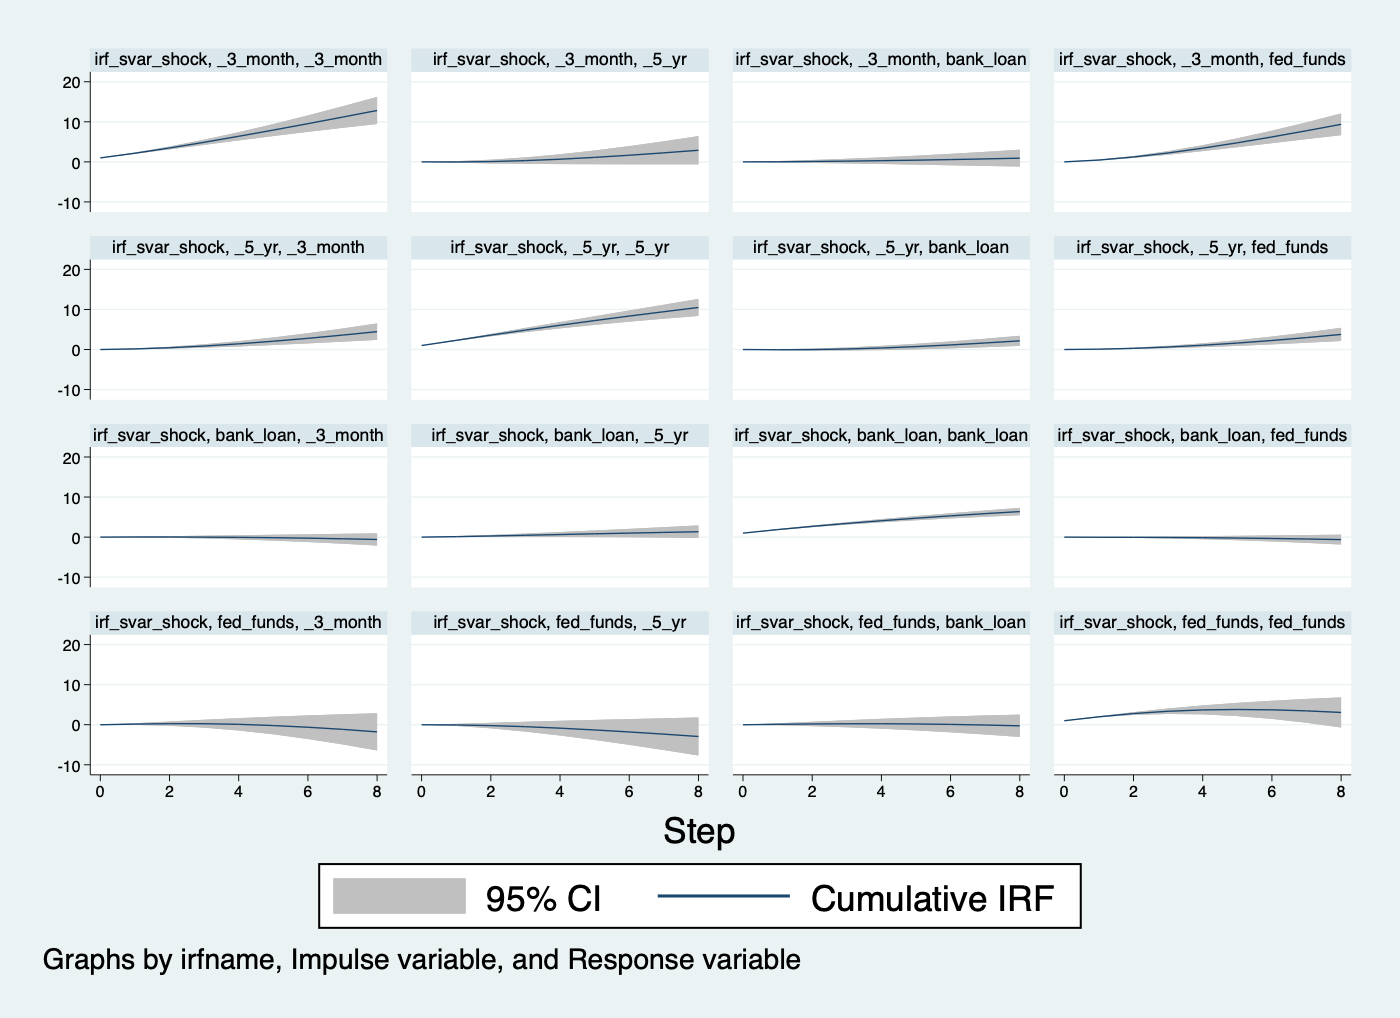
\includegraphics[width=5in]{irf_svar_shock.png} \\
The results are, again, what we would expect: there is a mostly positive relationship across the board when we look at the money and bond markets. We are particularly satisfied by seeing the 3-month and 5-year bonds following our exactly-predicted relationship. The bank loan market, however, seems to be the albatross, exhibiting a near-flat relationship with the federal funds impulse, a negative relationship with the 3-month impulse, and another near-flat relationship with the 5-year impulse. Perhaps this confusion is due to our selection of rate; it was difficult to find a bank loan rate that matched the rate Pétursson employed, and perhaps the finance rate on personal loans at commercial banks for a 24-month loan is \textit{not} effectively capturing the dynamics of the loan market.

Our results are similar to that of Pétursson; however, we want to note that Pétursson went beyond estimating the coefficients in his reduced-form model; he then estimates the over-identified system, incorporating complications and non-linearities in the reaction of the bank loan rate to shocks in other interest rates. He also engages in deep testing of his identifying assumptions, which we don't do. These areas would prove to be rich extensions of our research. 

\section{Conclusion}



We also went beyond a basic descriptive and cross-sectional approach, creating a structural VAR model to examine and test the impulse of the federal funds policy shocks--generated through its own VAR process--on shocks in sub-market rates. Overall, these findings matched our cross-sectional empirical findings, i.e., that the money and bond markets followed more closely monetary policy, while there was more disconnect between other segments of the financial system--such as housing, corporate bonds, and bank loaning. We look forward to extending this research with more robustness checks, continuing to flesh out our structural model through greater specification and identification tests (in particular mirroring Pétursson's work on over-identifying assumptions), and finally by incorporating dynamic term structural modeling (DTSM) that decompose and more closely analyze the term structure of the bonds that seem to be reacting so strongly to shocks in the federal funds rate. Finally, we would also be interested in extending this work to the Zero Lower Bound, and the Quantitative Easing (QE) programs the Federal Reserve engaged in during and in the wake of the Great Recession.

\clearpage
\bibliographystyle{ecta}
\bibliography{\bibfname}

\clearpage
\section{Appendix}
\subsection{VAR Estimations for Shocks}
The data on shocks for each respective rate is calculated using a basic VAR model and then subtracting the predicted values from the observed ones. Below are the tests for lag specification for each of the four rates of interest:
\begin{table}[!h]
\caption{Specification of the VAR 3-Month T-Bills}
\centering
\begin{tabular}{lllll}
\cline{1-5}
\multicolumn{1}{c}{} &
  \multicolumn{1}{|r}{AIC} &
  \multicolumn{1}{r}{SBIC} &
  \multicolumn{1}{r}{LL} &
  \multicolumn{1}{r}{LR} \\
\cline{1-5}
\multicolumn{1}{l}{k = 1} &
  \multicolumn{1}{|r}{-0.653} &
  \multicolumn{1}{r}{-0.630} &
  \multicolumn{1}{r}{109.385} &
  \multicolumn{1}{r}{79.473} \\
\multicolumn{1}{l}{k = 2} &
  \multicolumn{1}{|r}{-0.663} &
  \multicolumn{1}{r}{-0.628} &
  \multicolumn{1}{r}{112.003} &
  \multicolumn{1}{r}{5.237} \\
\multicolumn{1}{l}{k = 3} &
  \multicolumn{1}{|r}{-0.712} &
  \multicolumn{1}{r}{-0.665} &
  \multicolumn{1}{r}{121.057} &
  \multicolumn{1}{r}{18.107} \\
\multicolumn{1}{l}{k = 4} &
  \multicolumn{1}{|r}{-0.706} &
  \multicolumn{1}{r}{-0.649} &
  \multicolumn{1}{r}{121.209} &
  \multicolumn{1}{r}{0.305} \\
\cline{1-5}
\end{tabular}
\end{table}

\begin{table}[!h]
\caption{Specification of the VAR 5-Year T-Bonds}
\centering
\begin{tabular}{lllll}
\cline{1-5}
\multicolumn{1}{c}{} &
  \multicolumn{1}{|r}{AIC} &
  \multicolumn{1}{r}{SBIC} &
  \multicolumn{1}{r}{LL} &
  \multicolumn{1}{r}{LR} \\
\cline{1-5}
\multicolumn{1}{l}{k = 1} &
  \multicolumn{1}{|r}{-0.196} &
  \multicolumn{1}{r}{-0.173} &
  \multicolumn{1}{r}{34.271} &
  \multicolumn{1}{r}{28.946} \\
\multicolumn{1}{l}{k = 2} &
  \multicolumn{1}{|r}{-0.191} &
  \multicolumn{1}{r}{-0.156} &
  \multicolumn{1}{r}{34.388} &
  \multicolumn{1}{r}{0.235} \\
\multicolumn{1}{l}{k = 3} &
  \multicolumn{1}{|r}{-0.191} &
  \multicolumn{1}{r}{-0.144} &
  \multicolumn{1}{r}{35.358} &
  \multicolumn{1}{r}{1.940} \\
\multicolumn{1}{l}{k = 4} &
  \multicolumn{1}{|r}{-0.186} &
  \multicolumn{1}{r}{-0.129} &
  \multicolumn{1}{r}{35.638} &
  \multicolumn{1}{r}{0.560} \\
\cline{1-5}
\end{tabular}
\end{table}

\begin{table}[!h]
\caption{Specification of the VAR Bank Loans}
\centering
\begin{tabular}{lllll}
\cline{1-5}
\multicolumn{1}{c}{} &
  \multicolumn{1}{|r}{AIC} &
  \multicolumn{1}{r}{SBIC} &
  \multicolumn{1}{r}{LL} &
  \multicolumn{1}{r}{LR} \\
\cline{1-5}
\multicolumn{1}{l}{k = 1} &
  \multicolumn{1}{|r}{-0.265} &
  \multicolumn{1}{r}{-0.242} &
  \multicolumn{1}{r}{45.664} &
  \multicolumn{1}{r}{0.003} \\
\multicolumn{1}{l}{k = 2} &
  \multicolumn{1}{|r}{-0.259} &
  \multicolumn{1}{r}{-0.225} &
  \multicolumn{1}{r}{45.666} &
  \multicolumn{1}{r}{0.003} \\
\multicolumn{1}{l}{k = 3} &
  \multicolumn{1}{|r}{-0.403} &
  \multicolumn{1}{r}{-0.357} &
  \multicolumn{1}{r}{70.343} &
  \multicolumn{1}{r}{49.354} \\
\multicolumn{1}{l}{k = 4} &
  \multicolumn{1}{|r}{-0.397} &
  \multicolumn{1}{r}{-0.340} &
  \multicolumn{1}{r}{70.359} &
  \multicolumn{1}{r}{0.031} \\
\cline{1-5}
\end{tabular}
\end{table}

\begin{table}[!h]
\caption{Specification of the VAR Federal Funds}
\centering
\begin{tabular}{lllll}
\cline{1-5}
\multicolumn{1}{c}{} &
  \multicolumn{1}{|r}{AIC} &
  \multicolumn{1}{r}{SBIC} &
  \multicolumn{1}{r}{LL} &
  \multicolumn{1}{r}{LR} \\
\cline{1-5}
\multicolumn{1}{l}{k = 1} &
  \multicolumn{1}{|r}{-1.293} &
  \multicolumn{1}{r}{-1.270} &
  \multicolumn{1}{r}{214.715} &
  \multicolumn{1}{r}{199.799} \\
\multicolumn{1}{l}{k = 2} &
  \multicolumn{1}{|r}{-1.298} &
  \multicolumn{1}{r}{-1.263} &
  \multicolumn{1}{r}{216.466} &
  \multicolumn{1}{r}{3.503} \\
\multicolumn{1}{l}{k = 3} &
  \multicolumn{1}{|r}{-1.308} &
  \multicolumn{1}{r}{-1.261} &
  \multicolumn{1}{r}{219.107} &
  \multicolumn{1}{r}{5.281} \\
\multicolumn{1}{l}{k = 4} &
  \multicolumn{1}{|r}{-1.302} &
  \multicolumn{1}{r}{-1.244} &
  \multicolumn{1}{r}{219.111} &
  \multicolumn{1}{r}{0.009} \\
\cline{1-5}
\end{tabular}
\end{table}
 \\
In accordance with these results, we selected a lag of 3 for the 3-Month, 1 for the 5-Year, 3 for the bank loans, and 3 for the federal funds when running their univariate regressions. It may also be interesting and instructive to compare our estimates of monetary policy shocks to those of \citep{Acosta2022}: \\
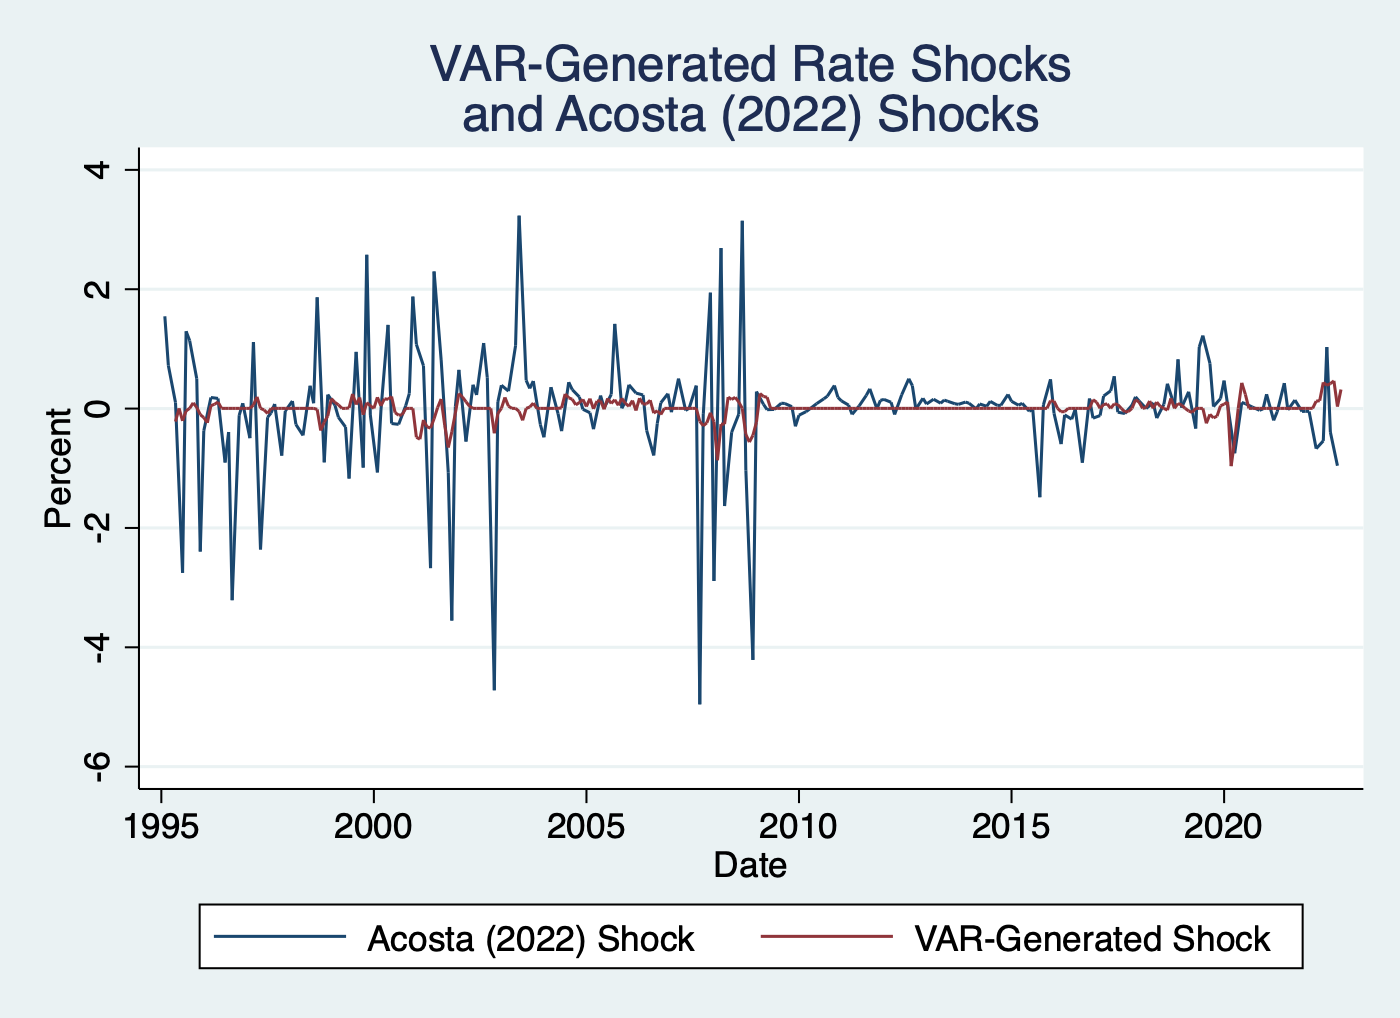
\includegraphics[width=5in]{shock_comparison.png}

\subsection{Péturrson's Derivation of the Wold Causal Chain}
In the main body of the paper, we largely skipped over how Pétursson derives the Wold Causal Chain that's used to estimate the structural VAR model. Below is a brief description summarizing his derivation of the SVAR model in his paper: we begin by creating a vector $x_t$ of our four variables of interest: $r_t$, $m_t$, $g_t$, and $b_t$. The VAR model is constructed of the following equations:
\begin{gather}
	C(L)x_t = e_t , \quad \quad \quad C_0 = I , \quad \quad \quad E(e_t e_t') = \Sigma
\end{gather}
Where we define $C(L)$ as a polynomial of a lag operator defined as $L^sx_t = x_{t-s}$, and $e_t$ is the one-stepped ahead forecast errors of $x_t$,  where the forecasts are merely predicted by the information provided by the lagged values of $x_t$. The equation (1) is merely a reduced-form relationship, however, and the power of structural estimation is given by the economic restrictions placed on our variables, which are given by the following equations:
\begin{gather}
	A(L)x_t = \epsilon_t, \quad \quad \quad E(\epsilon_t \epsilon_t ') = \Omega = \text{diag}(\omega_j^2)
\end{gather}
where $\epsilon_t$ is a vector of behavioral shocks, given by the following relation:
\begin{gather}
	A_0 e_t = \epsilon_t
\end{gather}
where $e_t$ is the VAR innovations of the variables in our information set and $A_0$ is the correlations (given by a matrix) among the information set's variables of interest. Therefore we can impose the following covariance structure on $e_t$, the VAR innovations:
\begin{gather}
	\Sigma = A_0^{-1}  \Omega  A_0^{-1\prime}
\end{gather}
In short, we need to estimate $n(n+1)/2$ parameters in equation (8), where $n$ is the number of variables in our information set (for us, it's 4). When we normalize the diagonal of $A_0$, which we recall is a matrix of correlations, we find that we actually need only $n(n-1)/2 = 4(3)/2 = 6$ restrictions, as described by our simple linear model outline in part 5.1 and equations (1) - (4). 

\end{document}